\chapter{Frey Microwave Auditory Effect}
\label{ch:frey-microwave-auditory-effect}

\begin{nontechnical}
\textbf{The Frey effect is hearing without sound}---when pulsed microwaves hit your head, you hear clicks or buzzes, but there's no actual sound in the air.

\textbf{Simple idea:}
\begin{itemize}
\item Pulsed microwaves $\rightarrow$ tiny, rapid heating
\item Heating $\rightarrow$ tissue expansion
\item Expansion $\rightarrow$ pressure wave inside head
\item Pressure wave $\rightarrow$ your ear detects it as sound
\end{itemize}

\textbf{Real use:} Discovered in 1962 near radar installations. Studied for communication systems and non-lethal weapons.

\textbf{Why you can hear it:} The pressure wave reaches your inner ear (cochlea) just like regular sound, but it's generated inside your head by electromagnetic energy, not by vibrating air outside.
\end{nontechnical}

\section{Overview}

The \textbf{Frey microwave auditory effect} (also called \textbf{microwave hearing} or \textbf{RF hearing}) is the perception of auditory sensations when exposed to \textbf{pulsed microwave radiation} at frequencies typically between 1--10~GHz. The effect occurs \textbf{without external sound}---the perception arises from \textbf{thermoelastic expansion} in tissue near the cochlea.

\begin{keyconcept}
The Frey effect demonstrates direct electromagnetic-to-acoustic transduction in biological tissue. Unlike conventional hearing (airborne sound), the acoustic pressure wave is generated \textbf{inside the head} by rapid microwave-induced heating, making it a unique biophysical phenomenon with applications in covert communication and non-lethal weapons.
\end{keyconcept}

\textbf{Key characteristics:}
\begin{itemize}
\item Requires \textbf{pulsed} microwaves (CW ineffective)
\item Perceived frequency matches pulse repetition rate, not carrier frequency
\item Threshold: $\sim$1--10~$\mu$J/cm$^2$ per pulse (very low energy)
\item Mechanism: Rapid heating $\rightarrow$ acoustic pressure wave $\rightarrow$ cochlear stimulation
\item Peak sensitivity at $\sim$2.45~GHz (ISM band)
\end{itemize}

\section{Discovery and Historical Background}

\subsection{Allan Frey's Original Experiments (1962)}

Allan Frey, a biophysicist, first reported the phenomenon after observing that personnel near radar installations heard auditory sensations synchronized with radar pulses \cite{Frey1962}.

\textbf{Controlled experiment:}
\begin{itemize}
\item Subjects exposed to pulsed microwaves at 1.3~GHz
\item Pulse duration: $\sim$10~$\mu$s, repetition rate: 100--1000~pps
\item Auditory perception reported as ``clicks'' or ``buzzing''
\item \textbf{Deaf subjects} with conductive hearing loss could perceive the effect
\item Sensorineural deaf individuals (cochlear damage) did \textbf{not} perceive it
\item Sound localized to head, not external space
\end{itemize}

\textbf{Frey's conclusion:} Microwaves directly stimulate the auditory system, bypassing the external ear.

\begin{calloutbox}{Historical Context}
Initial skepticism dismissed the effect as electromagnetic interference with equipment or auditory nerves. The phenomenon was later confirmed by multiple independent laboratories in the 1970s, establishing thermoelastic expansion as the mechanism \cite{Lin1980, Foster1974}.
\end{calloutbox}

\subsection{Subsequent Military Research (1970s--1990s)}

Declassified U.S. military studies confirmed the Frey effect in both animals and humans:
\begin{itemize}
\item Explored for ``voice-to-skull'' communication
\item Investigated for non-lethal weapon applications
\item Confirmed effect requires intact cochlea (ruled out direct neural stimulation)
\item Established perceived frequency matches pulse repetition rate
\item Identified peak sensitivity at $\sim$2.45~GHz
\end{itemize}

\section{Mathematical Description}

The Frey effect can be modeled quantitatively using thermoacoustic theory. The fundamental relationship between incident electromagnetic energy and generated acoustic pressure is:

\begin{equation}
p(t) = \frac{\beta \cdot c_s}{\rho_0 \cdot c_p} \cdot \frac{\partial}{\partial t}\left[\int_0^t \text{SAR}(\tau) \, d\tau\right]
\end{equation}
where:
\begin{itemize}
\item $p(t)$ = acoustic pressure (Pa)
\item $\beta$ = volumetric thermal expansion coefficient (K$^{-1}$)
\item $c_s$ = speed of sound in tissue (m/s)
\item $\rho_0$ = tissue density (kg/m$^3$)
\item $c_p$ = specific heat capacity (J/(kg·K))
\item SAR($\tau$) = specific absorption rate (W/kg)
\end{itemize}

For a short pulse with duration $\tau$ and constant SAR during the pulse:
\begin{equation}
p_{\text{max}} = \frac{\beta \cdot c_s}{\rho_0 \cdot c_p} \cdot \text{SAR} \cdot \tau
\end{equation}

This equation reveals that pressure amplitude is proportional to both pulse energy ($\text{SAR} \cdot \tau$) and the rate of energy deposition (shorter pulses at fixed energy produce higher pressure).

\section{Physical Mechanism: Thermoelastic Expansion}

\subsection{Step-by-Step Process}

\textbf{Step 1: Microwave absorption}

Pulsed microwave energy is absorbed by tissue, primarily water:
\begin{equation}
\text{Penetration depth} \quad \delta = \frac{1}{\alpha} \approx 1\text{--}3~\text{cm at 1--10~GHz}
\end{equation}
where $\alpha$ is the absorption coefficient (m$^{-1}$).

\textbf{Step 2: Rapid heating}

Pulse duration ($\tau \sim 1\text{--}10~\mu$s) is much shorter than thermal diffusion time ($\sim$1~ms), causing localized heating:
\begin{equation}
\Delta T = \frac{\text{SAR} \cdot \tau}{c_p}
\end{equation}
where:
\begin{itemize}
\item SAR = Specific Absorption Rate (W/kg)
\item $\tau$ = pulse duration (s)
\item $c_p \approx 3600$~J/(kg·K) = specific heat capacity of tissue
\end{itemize}

Temperature rise per pulse: $\Delta T \approx 10^{-6}$ to $10^{-5}$~K (imperceptibly small!).

\textbf{Step 3: Thermoelastic expansion}

Rapid heating causes tissue expansion before heat can diffuse away:
\begin{equation}
\frac{\Delta V}{V} = 3\alpha_T \Delta T
\end{equation}
where $\alpha_T \approx 3 \times 10^{-4}$~K$^{-1}$ is the thermal expansion coefficient.

The expansion occurs on the timescale of the pulse ($\sim\mu$s), launching an acoustic wave.

\textbf{Step 4: Acoustic propagation}

The pressure wave propagates through tissue to the cochlea at speed $c \approx 1500$~m/s:
\begin{equation}
p = \frac{\beta}{\rho_0 c_p} \cdot \text{SAR} \cdot \tau \cdot f_c
\end{equation}
where:
\begin{itemize}
\item $\beta \approx 10^{-4}$~K$^{-1}$ = thermal expansion coefficient
\item $\rho_0 \approx 1000$~kg/m$^3$ = tissue density
\item $f_c$ = microwave carrier frequency (Hz)
\item $p$ = acoustic pressure amplitude (Pa)
\end{itemize}

\textbf{Step 5: Cochlear detection}

Inner ear hair cells (stereocilia) detect the pressure wave and generate neural signals, which are processed by the auditory cortex as sound.

\subsection{Why Pulsed, Not CW?}

\textbf{Continuous Wave (CW) microwaves:}
\begin{itemize}
\item Produce steady heating
\item No rapid expansion-contraction cycles
\item No acoustic wave generation
\item \textbf{No auditory perception}
\end{itemize}

\textbf{Pulsed microwaves:}
\begin{itemize}
\item Rapid on-off creates expansion-contraction
\item Each pulse launches acoustic transient
\item Pulse train creates perceived tone at repetition rate
\item Pulse duration must be shorter than thermal diffusion time ($\sim$1~ms)
\end{itemize}

\begin{warningbox}
The pulse duration must satisfy $\tau \ll \tau_{\text{thermal}} \approx 1$~ms for efficient acoustic wave generation. Longer pulses allow heat to diffuse before expansion completes, dramatically reducing pressure amplitude.
\end{warningbox}

\section{Quantitative Analysis}

\subsection{Thermoelastic Pressure Generation}

Following the Lin \& Wang model \cite{Lin1980}, the peak acoustic pressure generated by a microwave pulse is:
\begin{equation}
p_{\text{peak}} = \frac{\beta \cdot \text{SAR} \cdot \tau}{c_p \cdot \rho_0 \cdot c_s}
\end{equation}
where $c_s \approx 1500$~m/s is the speed of sound in tissue.

\textbf{For typical parameters:}
\begin{itemize}
\item SAR $= 1$~W/kg
\item $\tau = 1~\mu$s
\item $\beta = 3 \times 10^{-4}$~K$^{-1}$
\item $c_p = 3600$~J/(kg·K)
\item $\rho_0 = 1000$~kg/m$^3$
\item $c_s = 1500$~m/s
\end{itemize}

\begin{equation}
p_{\text{peak}} = \frac{(3 \times 10^{-4})(1)(10^{-6})}{(3600)(1000)(1500)} \approx 5.6 \times 10^{-14}~\text{Pa}
\end{equation}

This is far below the hearing threshold ($\sim$20~$\mu$Pa). However, \textbf{focusing effects} near the cochlea and \textbf{resonant amplification} in the ear canal increase the effective pressure by several orders of magnitude.

\subsection{Hearing Threshold}

The human hearing threshold at 1~kHz is:
\begin{equation}
p_{\text{threshold}} \approx 20~\mu\text{Pa} = 2 \times 10^{-5}~\text{Pa} \quad (0~\text{dB SPL})
\end{equation}

\textbf{Energy threshold} for Frey effect perception:
\begin{equation}
E_{\text{threshold}} \approx 1\text{--}10~\mu\text{J/cm}^2~\text{per pulse}
\end{equation}

For a 1\% duty cycle (100~pps at 1~$\mu$s):
\begin{equation}
P_{\text{avg}} = E_{\text{threshold}} \cdot \text{PRF} \approx (10~\mu\text{J/cm}^2)(100~\text{s}^{-1}) = 0.1~\text{mW/cm}^2
\end{equation}

This is \textbf{well below} IEEE safety limits ($\sim$10~mW/cm$^2$ occupational).

\section{Frequency and Pulse Parameter Dependence}

\subsection{Carrier Frequency Dependence}

\begin{center}
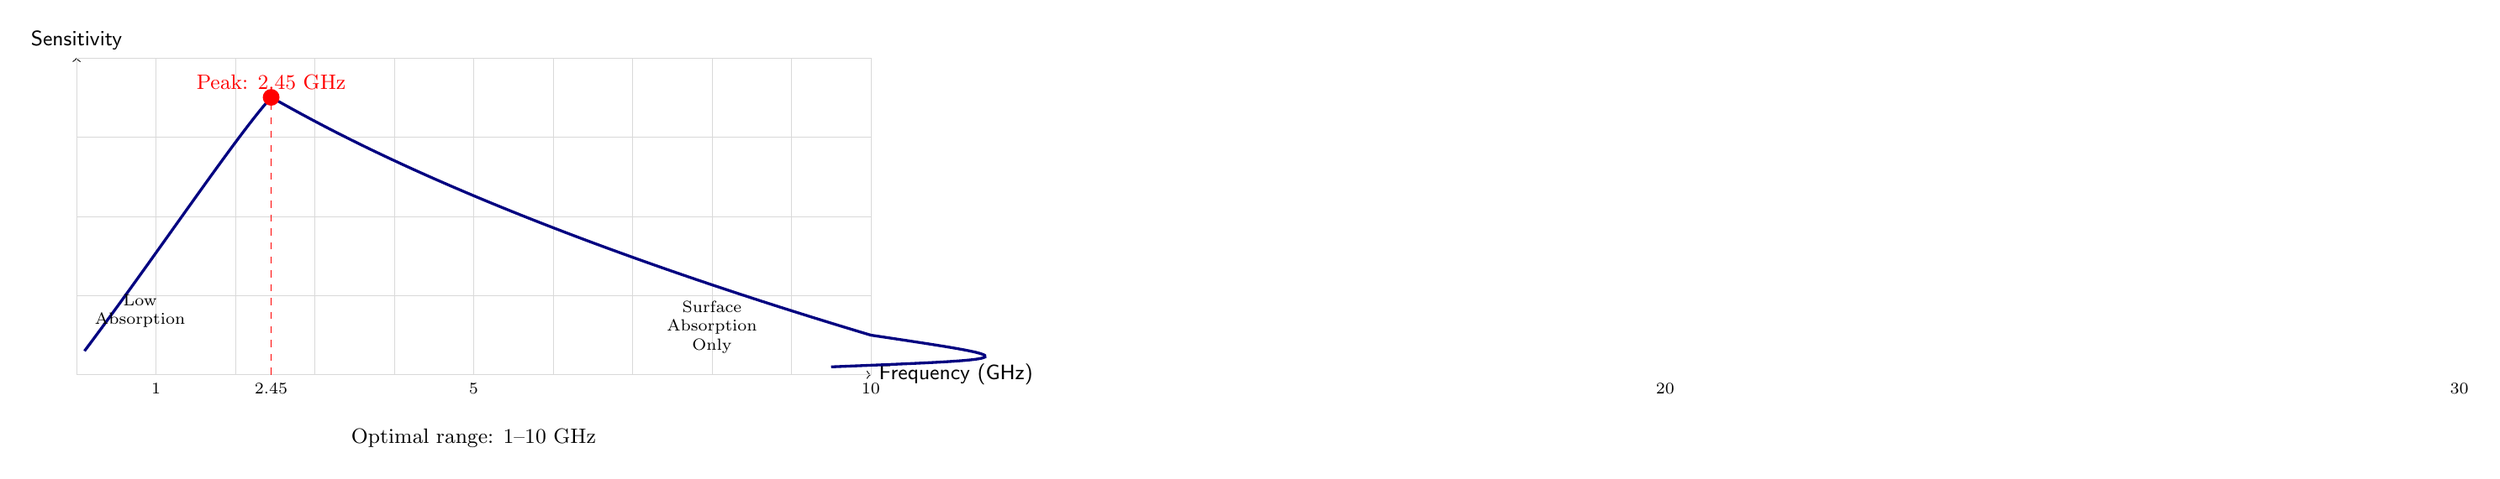
\begin{tikzpicture}[scale=1.2]
% Axes
\draw[->] (0,0) -- (10,0) node[right,font=\sffamily\small] {Frequency (GHz)};
\draw[->] (0,0) -- (0,4) node[above,font=\sffamily\small] {Sensitivity};

% Grid
\draw[very thin,gray!30] (0,0) grid[step=1] (10,4);

% Frequency markers
\foreach \x/\label in {1/1, 2.45/2.45, 5/5, 10/10, 20/20, 30/30}
  \node[below,font=\scriptsize] at (\x,0) {\label};

% Sensitivity curve (peak at 2.45 GHz)
\draw[very thick, NavyBlue] 
  (0.1,0.3) .. controls (1,1.5) and (2,3) .. (2.45,3.5)
  .. controls (3,3.2) and (5,2) .. (10,0.5)
  .. controls (12,0.2) .. (9.5,0.1);

% Peak marker
\fill[red] (2.45,3.5) circle (3pt);
\draw[dashed, red] (2.45,0) -- (2.45,3.5);
\node[above,font=\small,red] at (2.45,3.5) {Peak: 2.45~GHz};

% Regions
\node[font=\scriptsize,align=center] at (0.8,0.8) {Low\\Absorption};
\node[font=\scriptsize,align=center] at (8,0.6) {Surface\\Absorption\\Only};

% Labels
\node[font=\small,align=center] at (5,-0.8) {Optimal range: 1--10~GHz};
\end{tikzpicture}
\end{center}

\textbf{Frequency dependence:}
\begin{itemize}
\item \textbf{Below 100~MHz:} Penetrates too deeply, low absorption in head $\rightarrow$ weak effect
\item \textbf{1--10~GHz:} Optimal balance between penetration and absorption
\item \textbf{Peak at $\sim$2.45~GHz:} Coincides with maximum brain absorption
\item \textbf{Above 30~GHz:} Absorbed at skin surface, doesn't reach cochlea
\end{itemize}

\subsection{Pulse Duration Dependence}

\textbf{Optimal range:} 1--100~$\mu$s

\begin{itemize}
\item \textbf{Shorter ($<$1~$\mu$s):} Lower total energy, weaker acoustic wave
\item \textbf{Longer ($>$1~ms):} Heat diffuses before expansion completes, less efficient pressure generation
\item \textbf{Optimal:} Comparable to acoustic period ($\sim$10~$\mu$s for 100~kHz equivalent)
\end{itemize}

\subsection{Pulse Repetition Frequency (PRF)}

\textbf{PRF determines perceived pitch:}

\begin{center}
\begin{tabular}{@{}cl@{}}
\toprule
\textbf{PRF} & \textbf{Perceived Sound} \\
\midrule
10~Hz & Low rumble/hum \\
100~Hz & Buzz \\
1~kHz & Audible tone \\
10~kHz & High-pitched whistle \\
20~kHz & Approaching ultrasound limit \\
\bottomrule
\end{tabular}
\end{center}

\textbf{Audible range:} 20~Hz -- 20~kHz (same as acoustic hearing)

\begin{keyconcept}
The \textbf{carrier frequency} determines penetration and absorption, but the \textbf{pulse repetition frequency} determines the perceived pitch. A 2.45~GHz carrier pulsed at 1~kHz will be heard as a 1~kHz tone, not a 2.45~GHz ``note.''
\end{keyconcept}

\section{Performance Characteristics}

\subsection{Detection Threshold vs Frequency}

The threshold energy density for perception varies with carrier frequency, exhibiting a minimum at the optimal absorption frequency:

\begin{equation}
E_{\text{threshold}}(f) = E_{\text{min}} \cdot \left[1 + \left(\frac{f - f_{\text{opt}}}{f_{\text{bw}}}\right)^2\right]
\end{equation}
where:
\begin{itemize}
\item $E_{\text{min}} \approx 1~\mu$J/cm$^2$ at $f_{\text{opt}} = 2.45$~GHz
\item $f_{\text{bw}} \approx 5$~GHz is the effective bandwidth
\end{itemize}

\subsection{Power Efficiency}

The conversion efficiency from electromagnetic to acoustic energy is extremely low:
\begin{equation}
\eta_{\text{conversion}} = \frac{P_{\text{acoustic}}}{P_{\text{EM}}} \approx 10^{-9} \text{ to } 10^{-8}
\end{equation}

Despite this low efficiency, the human auditory system's exceptional sensitivity ($\sim$20~$\mu$Pa threshold) enables perception at safe EM exposure levels.

\subsection{Range-Power Trade-off}

For a target at distance $d$ with required energy density $E$:
\begin{equation}
P_{\text{TX}} = \frac{4\pi d^2 \cdot E \cdot A}{\tau \cdot G_t \cdot G_r}
\end{equation}
where:
\begin{itemize}
\item $A$ = target cross-sectional area (m$^2$)
\item $G_t$, $G_r$ = transmit and receive antenna gains
\item $\tau$ = pulse duration
\end{itemize}

This $d^2$ dependence severely limits practical range for portable systems.

\section{Experimental Evidence}

\subsection{Human Psychophysics}

Guy et al. (1975) \cite{Guy1975} measured thresholds across the frequency range:

\begin{center}
\begin{tabular}{@{}lrr@{}}
\toprule
\textbf{Frequency} & \textbf{Threshold} & \textbf{Avg Power (1\% duty)} \\
\midrule
200~MHz & 25~$\mu$J/cm$^2$ & 0.25~mW/cm$^2$ \\
915~MHz & 5~$\mu$J/cm$^2$ & 0.05~mW/cm$^2$ \\
\textbf{2.45~GHz} & \textbf{1~$\mu$J/cm$^2$} & \textbf{0.01~mW/cm$^2$} \\
10~GHz & 8~$\mu$J/cm$^2$ & 0.08~mW/cm$^2$ \\
\bottomrule
\end{tabular}
\end{center}

\textbf{Perceived sound characteristics:}
\begin{itemize}
\item \textbf{Single pulse:} Click
\item \textbf{10--100~pps:} Buzz
\item \textbf{$>$1000~pps:} Tone at PRF frequency
\item \textbf{CW exposure:} No sound (even at high power)
\end{itemize}

\subsection{Animal Studies}

\textbf{Cochlear microphonics} (Elder \& Chou, 2003) \cite{Elder2003}:
\begin{itemize}
\item Microelectrode placed in guinea pig cochlea
\item Pulsed microwaves evoked electrical signals matching pulse rate
\item Signal abolished by cochlear destruction
\item \textbf{Conclusion:} Direct evidence for cochlear transduction
\end{itemize}

\textbf{Auditory brainstem response (ABR):}
\begin{itemize}
\item EEG-like measurement of auditory pathway
\item Pulsed microwaves evoke ABR similar to acoustic clicks
\item Latency and waveform consistent with acoustic stimulation
\end{itemize}

\subsection{Deaf Subject Studies}

\begin{center}
\begin{tabular}{@{}lcc@{}}
\toprule
\textbf{Type of Deafness} & \textbf{Perceive Effect?} & \textbf{Implication} \\
\midrule
Conductive (middle ear damage) & \checkmark Yes & Bypasses external/middle ear \\
Sensorineural (cochlear damage) & \texttimes No & Requires intact cochlea \\
Normal hearing & \checkmark Yes & Baseline confirmation \\
\bottomrule
\end{tabular}
\end{center}

\textbf{Conclusion:} The effect requires intact cochlear hair cells but does not require functioning middle ear ossicles. This confirms the acoustic pressure wave reaches the cochlea through tissue, not air.

\section{Block Diagram of the Frey Effect}

\begin{center}
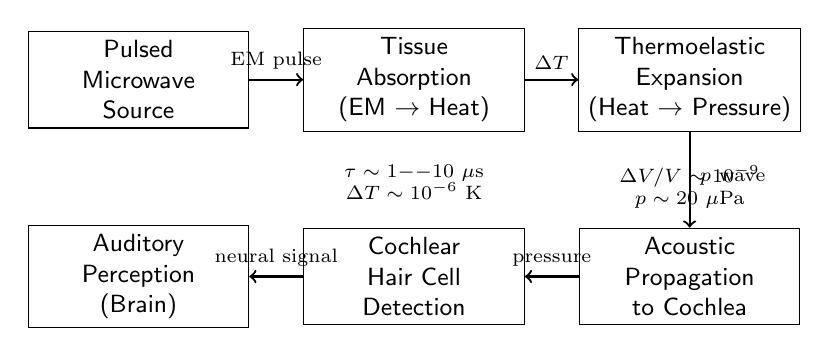
\begin{tikzpicture}[
  block/.style={rectangle, draw, minimum width=2.8cm, minimum height=1.2cm, font=\sffamily\small, align=center},
  node distance=2.5cm,
  font=\small
]

% Blocks
\node[block] (source) {Pulsed\\Microwave\\Source};
\node[block, right of=source, node distance=3.5cm] (absorb) {Tissue\\Absorption\\(EM $\rightarrow$ Heat)};
\node[block, right of=absorb, node distance=3.5cm] (expand) {Thermoelastic\\Expansion\\(Heat $\rightarrow$ Pressure)};
\node[block, below of=expand, node distance=2.5cm] (propagate) {Acoustic\\Propagation\\to Cochlea};
\node[block, left of=propagate, node distance=3.5cm] (detect) {Cochlear\\Hair Cell\\Detection};
\node[block, left of=detect, node distance=3.5cm] (percept) {Auditory\\Perception\\(Brain)};

% Connections
\draw[->, thick] (source) -- node[above,font=\scriptsize] {EM pulse} (absorb);
\draw[->, thick] (absorb) -- node[above,font=\scriptsize] {$\Delta T$} (expand);
\draw[->, thick] (expand) -- node[right,font=\scriptsize] {$p$ wave} (propagate);
\draw[->, thick] (propagate) -- node[above,font=\scriptsize] {pressure} (detect);
\draw[->, thick] (detect) -- node[above,font=\scriptsize] {neural signal} (percept);

% Annotations
\node[font=\scriptsize,align=center,below=0.3cm] at (absorb.south) {$\tau \sim 1\text{--}10~\mu$s\\$\Delta T \sim 10^{-6}$~K};
\node[font=\scriptsize,align=center,below=0.3cm] at (expand.south) {$\Delta V/V \sim 10^{-9}$\\$p \sim 20~\mu$Pa};

\end{tikzpicture}
\end{center}

\section{Safety Considerations}

\subsection{Exposure Limits vs Frey Threshold}

\textbf{IEEE/ICNIRP safety guidelines:}
\begin{itemize}
\item \textbf{Occupational:} 10~mW/cm$^2$ (averaged over 6 minutes)
\item \textbf{General public:} 2~mW/cm$^2$
\item Based on \textbf{thermal effects} (tissue heating)
\end{itemize}

\textbf{Frey effect threshold:}
\begin{itemize}
\item Energy: $\sim$1--10~$\mu$J/cm$^2$ per pulse
\item For 1~$\mu$s pulse at 100~pps: Average power $\approx$ 0.01~mW/cm$^2$
\item \textbf{100$\times$ below occupational safety limit}
\end{itemize}

\begin{importantbox}
The Frey effect can occur at exposures considered safe for thermal damage. The perception is \textbf{non-hazardous} but can be \textbf{annoying or disorienting}, particularly for prolonged exposure or high pulse rates.
\end{importantbox}

\subsection{Health Effects}

\textbf{Acute effects:}
\begin{itemize}
\item Auditory perception (transient, reversible)
\item Annoyance, distraction, startle response
\item No tissue damage at threshold levels
\end{itemize}

\textbf{Chronic effects:}
\begin{itemize}
\item No known long-term effects from brief exposures at threshold
\item High-intensity repeated exposure could cause cochlear damage (acoustic trauma-like)
\item Equivalent to moderate sound exposure ($\sim$60--80~dB SPL)
\end{itemize}

\section{Worked Example: Frey Effect System Design}

\textbf{Problem:} Design a pulsed microwave system to demonstrate the Frey effect in a laboratory setting at a distance of 10~m, ensuring safety compliance while achieving audible perception.

\textbf{Given:}

\begin{tabular}{@{}ll@{}}
Target distance & $d = 10$~m \\
Required energy density & $E = 5~\mu$J/cm$^2$ per pulse (threshold) \\
Carrier frequency & $f_c = 2.45$~GHz (peak sensitivity) \\
Pulse duration & $\tau = 10~\mu$s \\
Pulse repetition frequency & PRF $= 1$~kHz (audible tone) \\
Transmit antenna gain & $G_t = 20$~dBi (horn antenna) \\
\end{tabular}

\textbf{Solution:}

\textbf{Step 1: Calculate Required Pulse Energy}

Target area: $A = 100$~cm$^2$ (head cross-section)

\begin{equation}
E_{\text{pulse}} = E \cdot A = (5~\mu\text{J/cm}^2)(100~\text{cm}^2) = 500~\mu\text{J} = 5 \times 10^{-4}~\text{J}
\end{equation}

\subsection*{Step 2: Calculate Peak Transmit Power}

\begin{equation}
P_{\text{peak}} = \frac{E_{\text{pulse}}}{\tau} = \frac{5 \times 10^{-4}~\text{J}}{10 \times 10^{-6}~\text{s}} = 50~\text{W}
\end{equation}

\subsection*{Step 3: Account for Free-Space Path Loss}

At distance $d = 10$~m and frequency $f_c = 2.45$~GHz:

\begin{equation}
\text{FSPL} = 20\log_{10}(d) + 20\log_{10}(f_{\text{MHz}}) + 32.45
\end{equation}
\begin{equation}
\text{FSPL} = 20\log_{10}(0.01) + 20\log_{10}(2450) + 32.45 = 60.2~\text{dB}
\end{equation}

\subsection*{Step 4: Calculate Required TX Power}

\begin{equation}
P_{\text{TX}} = P_{\text{peak}} + \text{FSPL} - G_t
\end{equation}
\begin{equation}
P_{\text{TX}} = 10\log_{10}(50) + 60.2 - 20 = 17.0 + 60.2 - 20 = 57.2~\text{dBm} \approx 525~\text{W}
\end{equation}

\subsection*{Step 5: Calculate Average Power}

Duty cycle: $DC = \tau \cdot \text{PRF} = (10~\mu\text{s})(1000~\text{s}^{-1}) = 0.01 = 1\%$

\begin{equation}
P_{\text{avg}} = P_{\text{peak}} \cdot DC = 525~\text{W} \times 0.01 = 5.25~\text{W}
\end{equation}

\begin{calloutbox}[colback=black!5!white,colframe=black]{Design Summary}
\textbf{System parameters:}
\begin{itemize}
\item Peak transmit power: 525~W (57~dBm)
\item Average power: 5.25~W (7.2~dBm)
\item Pulse duration: 10~$\mu$s
\item Pulse rate: 1~kHz (heard as 1~kHz tone)
\item Antenna: 20~dBi horn
\item Range: 10~m
\end{itemize}

\textbf{Safety check:}
\begin{itemize}
\item Average power density at target: $\approx 0.05$~mW/cm$^2$
\item IEEE limit (occupational): 10~mW/cm$^2$
\item \textbf{Margin: 200$\times$ below safety limit}
\end{itemize}

\textbf{Conclusion:} Frey effect demonstration is feasible with modest average power but requires high peak power magnetron or solid-state transmitter.
\end{calloutbox}

\section{Applications}

\subsection{Non-Lethal Weapons and Deterrents}

\textbf{Concept:} Direct pulsed microwaves at target to induce disorienting sounds (``voice in head'').

\textbf{Advantages:}
\begin{itemize}
\item[\checkmark] No physical projectile
\item[\checkmark] Reversible effect
\item[\checkmark] Can encode information (modulate PRF to transmit speech)
\item[\checkmark] Psychological impact
\end{itemize}

\textbf{Challenges:}
\begin{itemize}
\item[\texttimes] Requires high peak power (kW) $\rightarrow$ bulky equipment
\item[\texttimes] Line-of-sight only (microwaves don't penetrate walls at GHz)
\item[\texttimes] Ethical concerns (psychological effects)
\item[\texttimes] Limited range ($<$100~m typical)
\end{itemize}

\textbf{Status:} Prototypes exist (U.S. military ``MEDUSA'' system, DARPA 2008) but deployment status unclear.

\subsection{Covert Communication}

\textbf{Concept:} Transmit speech via modulated microwave pulses so only the target hears.

\textbf{Implementation:}
\begin{itemize}
\item Encode audio waveform in PRF modulation
\item Focus beam on target individual
\item Speech bandwidth: $\sim$300--3000~Hz (telephone quality)
\item Maximum PRF: $\sim$10~kHz (limited by audible range)
\end{itemize}

\textbf{Limitations:}
\begin{itemize}
\item Speech intelligibility limited by PRF bandwidth
\item Target must be stationary (beam focusing required)
\item Practical range: $<$50~m
\end{itemize}

\subsection{Assistive Hearing Devices (Proposed)}

\textbf{Concept:} For conductive deaf (damaged middle ear), bypass ossicles with microwave stimulation.

\textbf{Reality check:}
\begin{itemize}
\item[\checkmark] Works for conductive hearing loss
\item[\texttimes] Sensorineural deafness (damaged hair cells) eliminates effect
\item[\texttimes] Cochlear implants (electrical stimulation) are more effective
\item[\texttimes] Safety concerns for continuous exposure
\end{itemize}

\textbf{Status:} Not pursued due to superiority of cochlear implants.

\subsection{Brain Imaging and Research}

\textbf{Concept:} Use pulsed microwaves to selectively activate auditory cortex for fMRI mapping.

\textbf{Advantages over acoustic stimulation:}
\begin{itemize}
\item No MRI scanner acoustic noise interference
\item Precise temporal control
\item Bypasses external/middle ear confounds
\end{itemize}

\textbf{Status:} Not actively pursued due to ethical and safety concerns.

\section{Comparison to Related Phenomena}

\subsection{Acoustic Heterodyning}

\begin{center}
\begin{tabular}{@{}lll@{}}
\toprule
\textbf{Aspect} & \textbf{Frey Effect} & \textbf{Acoustic Heterodyning} \\
\midrule
Input & EM waves (microwaves) & Acoustic waves (ultrasound) \\
Mechanism & Thermoelastic expansion & Nonlinear wave mixing \\
Transduction & EM $\rightarrow$ acoustic & Acoustic $\rightarrow$ acoustic \\
Perception site & Inside head & External (in air) \\
Frequency range & 1--10~GHz carrier & 20--100~kHz ultrasound \\
Application & Covert communication & Directional speakers \\
\bottomrule
\end{tabular}
\end{center}

\textbf{Similarity:} Both create perceived sound ``from nothing'' (no conventional speaker).

\textbf{Difference:} Frey is EM-to-acoustic transduction; heterodyning is acoustic-to-acoustic.

\subsection{THz Bioeffects}

\textbf{THz frequencies} (0.1--10~THz) are $\sim$100--1000$\times$ higher than Frey effect microwaves (GHz).

\textbf{Could THz cause similar effect?}
\begin{itemize}
\item[\texttimes] \textbf{No:} THz absorbed at skin ($<$1~mm penetration), never reaches cochlea
\item Frey effect requires \textbf{volumetric heating} in tissue near cochlea
\item THz limited to surface effects
\end{itemize}

\section{Controversies and Misconceptions}

\subsection{``Mind Control'' and Conspiracy Theories}

\textbf{Misconception:} Frey effect can implant thoughts or control behavior.

\textbf{Reality:}
\begin{itemize}
\item Effect only creates auditory perception
\item Cannot write information directly to brain
\item No different from hearing sound via ears
\item No evidence of cognitive or behavioral effects beyond distraction
\end{itemize}

\subsection{``Havana Syndrome''}

\textbf{Background:} Unexplained health incidents (2016--present) involving U.S. diplomats attributed to ``sonic attacks'' or directed energy weapons.

\textbf{Possible explanations:}
\begin{itemize}
\item Pulsed microwaves (Frey effect)
\item Ultrasound
\item Mass psychogenic illness
\item Environmental factors (pesticides, crickets)
\end{itemize}

\textbf{Scientific consensus:} Mechanism unproven. Microwave explanation plausible but not confirmed. NAS report (2020) suggested ``directed pulsed RF energy'' as consistent with symptoms \cite{NAS2020}.

\subsection{5G and Cell Phones}

\textbf{Question:} Can 5G towers or cell phones cause Frey effect?

\textbf{Answer:} \textbf{No}
\begin{itemize}
\item Cell signals are CW or quasi-CW (not short pulses)
\item Power too low (milliwatts vs kilowatts needed)
\item Frequency sub-optimal (5G uses 3--30~GHz with limited penetration at high end)
\item No credible mechanism for sustained effect
\end{itemize}

\section{Signal Processing Diagram}

\begin{center}
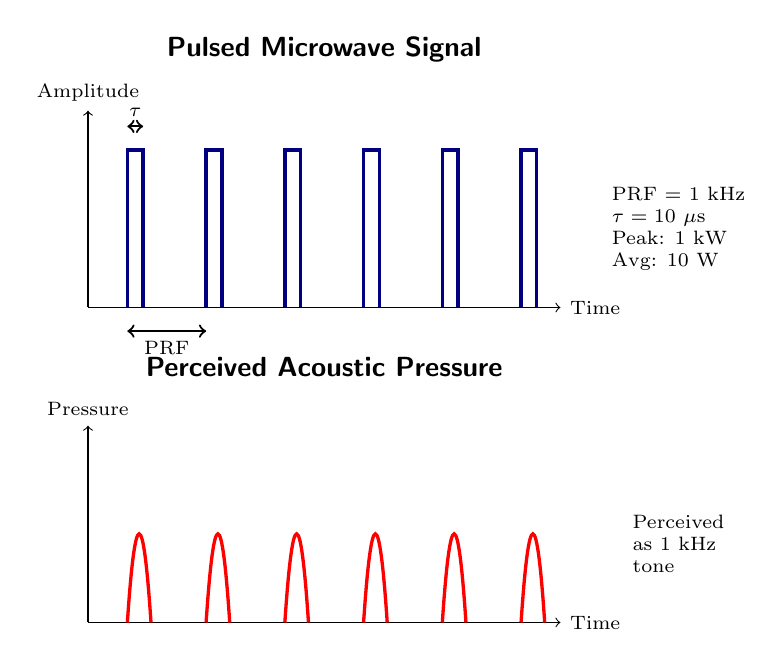
\begin{tikzpicture}[scale=1.0]
% Time domain representation
\begin{scope}[shift={(0,0)}]
\node[above,font=\sffamily\bfseries] at (3,3) {Pulsed Microwave Signal};

% Axes
\draw[->] (0,0) -- (6,0) node[right,font=\scriptsize] {Time};
\draw[->] (0,0) -- (0,2.5) node[above,font=\scriptsize] {Amplitude};

% Pulses
\foreach \x in {0.5, 1.5, 2.5, 3.5, 4.5, 5.5} {
  \draw[very thick, NavyBlue] (\x,0) -- (\x,2) -- (\x+0.2,2) -- (\x+0.2,0);
}

% Annotations
\draw[<->, thick] (0.5,-0.3) -- (1.5,-0.3) node[midway,below,font=\scriptsize] {PRF};
\draw[<->, thick] (0.5,2.3) -- (0.7,2.3) node[midway,above,font=\scriptsize] {$\tau$};

\node[font=\scriptsize,align=left] at (7.5,1) {PRF = 1~kHz\\$\tau = 10~\mu$s\\Peak: 1~kW\\Avg: 10~W};
\end{scope}

% Perceived acoustic signal
\begin{scope}[shift={(0,-4)}]
\node[above,font=\sffamily\bfseries] at (3,3) {Perceived Acoustic Pressure};

% Axes
\draw[->] (0,0) -- (6,0) node[right,font=\scriptsize] {Time};
\draw[->] (0,0) -- (0,2.5) node[above,font=\scriptsize] {Pressure};

% Acoustic pulses (broader)
\foreach \x in {0.5, 1.5, 2.5, 3.5, 4.5, 5.5} {
  \draw[very thick, red] (\x,0) .. controls (\x+0.1,1.5) and (\x+0.2,1.5) .. (\x+0.3,0);
}

% Annotation
\node[font=\scriptsize,align=left] at (7.5,1) {Perceived\\as 1~kHz\\tone};
\end{scope}

\end{tikzpicture}
\end{center}

\section{Advantages and Disadvantages}

\subsection*{Advantages}

\begin{enumerate}
\item \textbf{Non-invasive:} No physical contact or device implantation required
\item \textbf{Bypasses external/middle ear:} Effective for conductive hearing loss
\item \textbf{Covert capability:} Only target individual perceives signal
\item \textbf{Scientifically interesting:} Demonstrates EM-biological coupling
\item \textbf{Low average power:} Can operate below thermal safety limits
\end{enumerate}

\subsection*{Disadvantages}

\begin{enumerate}
\item \textbf{High peak power required:} Kilowatt-level transmitters needed
\item \textbf{Limited range:} Typically $<$100~m practical
\item \textbf{Line-of-sight only:} GHz microwaves don't penetrate walls
\item \textbf{Ethical concerns:} Potential for psychological impact
\item \textbf{Requires intact cochlea:} Ineffective for sensorineural deafness
\item \textbf{Speech quality limited:} PRF bandwidth constrains intelligibility
\end{enumerate}

\section{Summary}

\begin{center}
\begin{tabular}{@{}ll@{}}
\toprule
\textbf{Parameter} & \textbf{Value/Description} \\
\midrule
Phenomenon & Hearing without external sound \\
Mechanism & Thermoelastic expansion \\
Optimal frequency & 1--10~GHz (peak: 2.45~GHz) \\
Pulse duration & 1--100~$\mu$s \\
Energy threshold & 1--10~$\mu$J/cm$^2$ per pulse \\
Perceived frequency & Equals pulse repetition rate \\
Safety & Well below thermal damage limits \\
Discovery & Allan Frey, 1962 \\
Applications & Non-lethal weapons, covert comms \\
Limitation & Requires high peak power \\
\bottomrule
\end{tabular}
\end{center}

The Frey microwave auditory effect remains one of the most intriguing examples of electromagnetic-biological interaction. While its practical applications are limited by technical and ethical constraints, it demonstrates fundamental biophysical principles and continues to be relevant in discussions of directed energy weapons and unexplained auditory phenomena.

\section{Further Reading}

\begin{itemize}
\item \textbf{Thermoelastic Wave Propagation:} Acoustic wave generation in tissue
\item \textbf{Acoustic Heterodyning:} Parametric arrays and nonlinear acoustics
\item \textbf{Non-Linear Biological Demodulation:} EM-biology interactions
\item \textbf{Intermodulation Distortion in Biology:} Nonlinear mixing effects
\item \textbf{THz Bioeffects:} High-frequency EM interactions with tissue
\item \textbf{Directed Energy Weapons:} Military applications of high-power RF
\item \textbf{Cochlear Mechanics:} Inner ear transduction mechanisms
\end{itemize}

\begin{thebibliography}{99}
\bibitem{Frey1962} Frey, A. H. (1962). ``Human Auditory System Response to Modulated Electromagnetic Energy.'' \textit{Journal of Applied Physiology}, 17(4), 689--692.

\bibitem{Lin1980} Lin, J. C. (1980). ``The Microwave Auditory Phenomenon.'' \textit{Proceedings of the IEEE}, 68(1), 67--73.

\bibitem{Foster1974} Foster, K. R., \& Finch, E. D. (1974). ``Microwave Hearing: Evidence for Thermoacoustic Auditory Stimulation by Pulsed Microwaves.'' \textit{Science}, 185(4147), 256--258.

\bibitem{Guy1975} Guy, A. W., Chou, C. K., Lin, J. C., \& Christensen, D. (1975). ``Microwave-Induced Acoustic Effects in Mammalian Auditory Systems and Physical Materials.'' \textit{Annals of the New York Academy of Sciences}, 247, 194--218.

\bibitem{Elder2003} Elder, J. A., \& Chou, C. K. (2003). ``Auditory Response to Pulsed Radiofrequency Energy.'' \textit{Bioelectromagnetics}, 24(S6), S162--S173.

\bibitem{NAS2020} National Academies of Sciences, Engineering, and Medicine (2020). \textit{An Assessment of Illness in U.S. Government Employees and Their Families at Overseas Embassies}. Washington, DC: The National Academies Press.
\end{thebibliography}
